\documentclass[a4paper, 12pt]{article}


\usepackage[T1]{fontenc}      % Codificación de fuentes
\usepackage{cite}             % Para citar referencias
\usepackage[utf8]{inputenc} % Codificación de caracteres
\usepackage[spanish]{babel}  % Idioma español
\usepackage{amsmath}         % Paquete para matemáticas
\usepackage{graphicx}        % Para incluir imágenes
\usepackage{hyperref}        % Para enlaces
\usepackage{subcaption}
\usepackage{comment}

\title{Taller 1 Maquinas Electricas} % Título del documento
\author{Daniel Fernando Aranda Contreras} % Autor del documento
\date{\today} % Fecha actual, puedes cambiarla por una fecha específica

\begin{document}


\begin{abstract}
    Tales.
\end{abstract}

\section{OBJETIVOS }
Comprender las diferentes formas de conexion en el transformador para identificar los bornes, la resistencia de aislamiento, la relacion de transformacion y la polaridad de un transformador monofasico.
\newline
\\
Calcular la resistencia de aislamiento, la relacion de transformacion y conocer cual es la polaridad de un transformador monofasico.
\newline
\\
Describir los metodos empleados en la practica y el Desarrollo del calculo.
\newline
\\
Explorar los metodos no empleados en la practica para la determinacion de la polaridad de un transformador monofasico y el calculo de la resistencia de aislamiento mediante el metodo indirecto.
\newpage
\section{EQUIPOS Y MATERIALES}
\begin{figure}[h] % 'h' indica que la imagen se coloca aquí
    \centering
    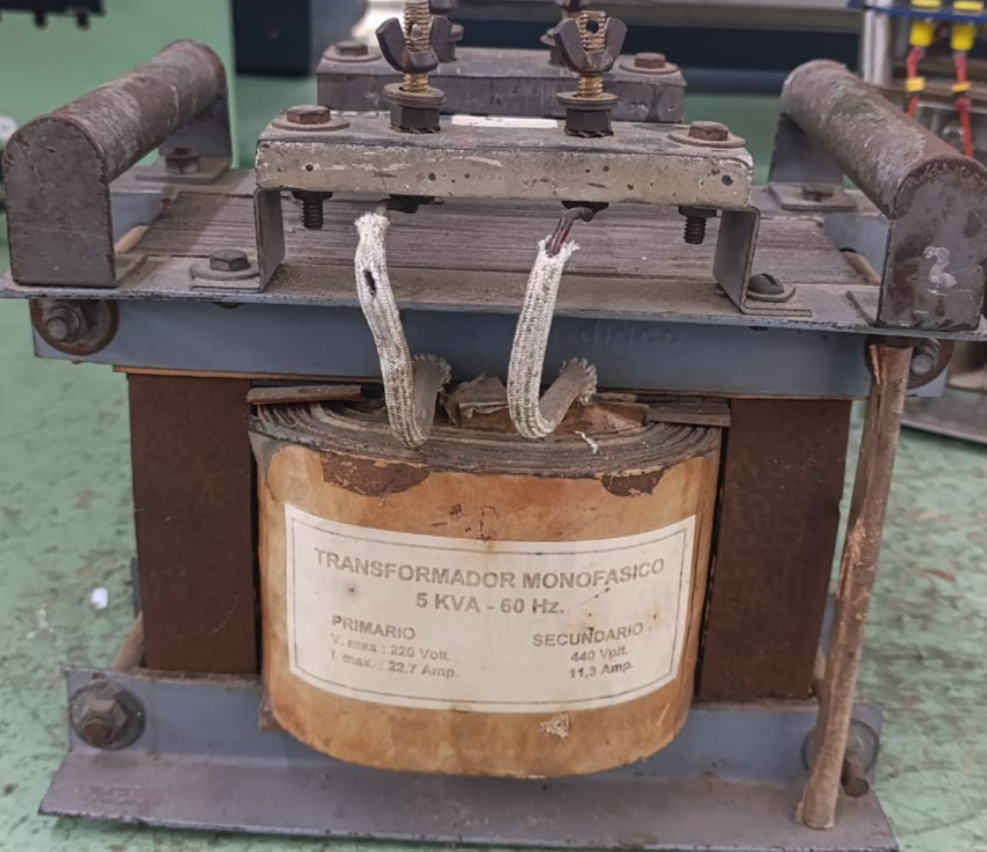
\includegraphics[width=0.5\textwidth]{img/Transformador monofasico.png} % Cambia la ruta a tu imagen
    \caption{Ficha tecnica del transformador monofasico.}
    \label{fig:mi_imagen}
\end{figure}
\begin{figure}[h] % 'h' indica que la imagen se coloca aquí
    \centering
    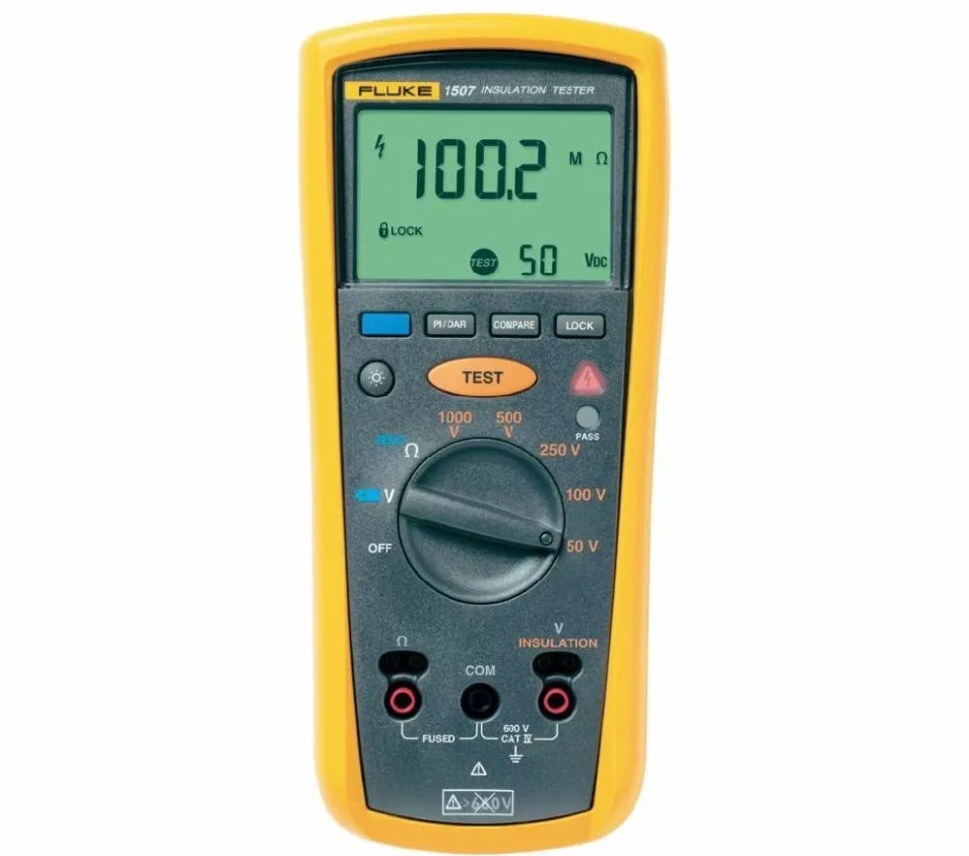
\includegraphics[width=0.5\textwidth]{img/Megahometro megger.png} % Cambia la ruta a tu imagen
    \caption{Megahometro Fluke 1507.}
    \label{fig:megahometro}
\end{figure}
\begin{figure}[h] % 'h' indica que la imagen se coloca aquí
    \centering
    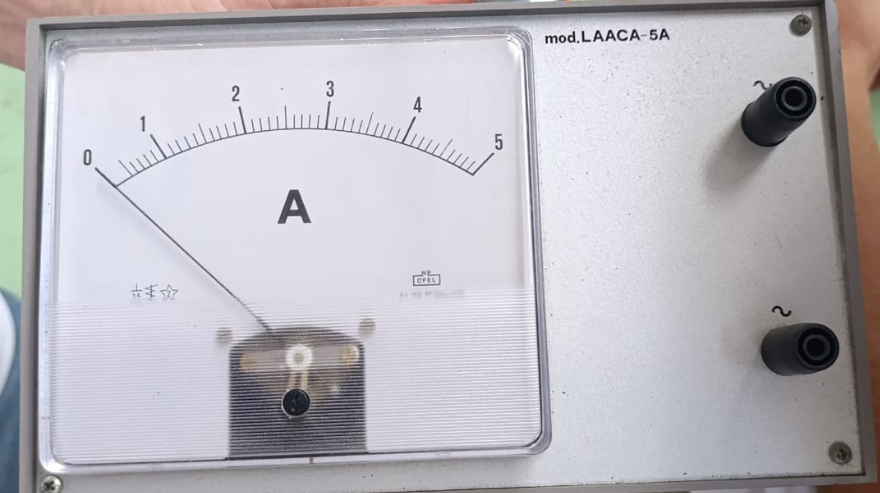
\includegraphics[width=0.5\textwidth]{img/Amperimetro Analogico.png} % Cambia la ruta a tu imagen
    \caption{Amperimetro Analogico.}
    \label{fig:AmpAnalogico}
\end{figure}
\begin{figure}[h] % 'h' indica que la imagen se coloca aquí
    \centering
    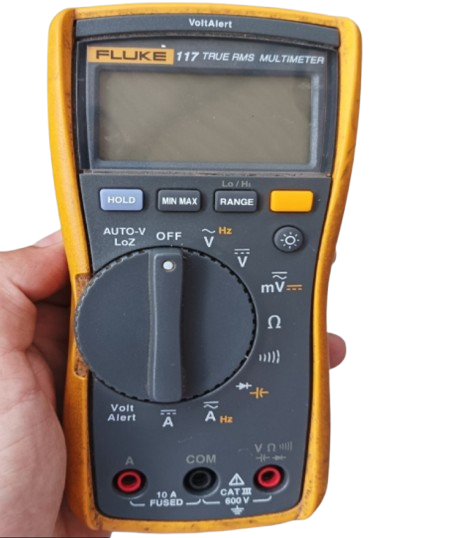
\includegraphics[width=0.5\textwidth]{img/Multimetro digital.png} % Cambia la ruta a tu imagen
    \caption{Multimetro Fluke 117.}
    \label{fig:MulDigital}
\end{figure}



\begin{comment}
    Este es un bloque de texto comentado.

\begin{verbatim}
    int main() {
        printf("Hola, mundo!");
        return 0;
    }
    \end{verbatim}
    
    \begin{figure}[ht!]
        \centering
        \subfloat[Ficha tecnica del transformador monofasico.]{%
            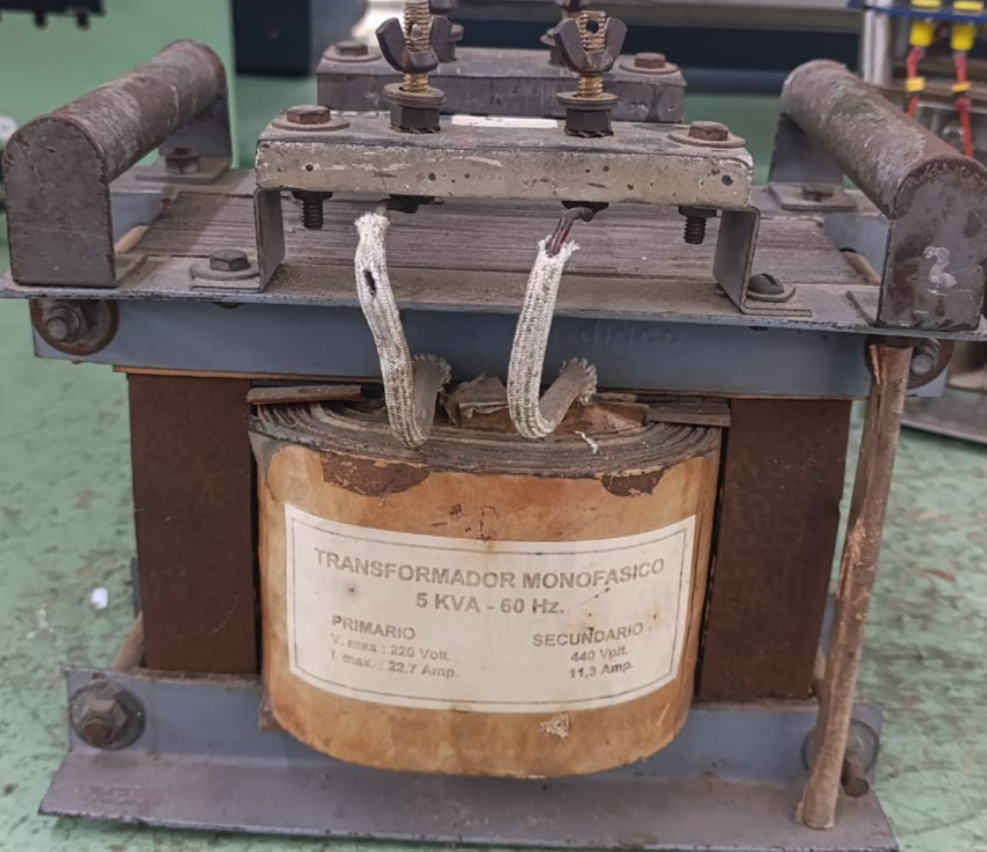
\includegraphics[width=0.3\textwidth]{img/Transformador monofasico.png}%
            \label{fig:imagen1}
        }\hfill
        \subfloat[Megahometro Fluke 1507.]{%
            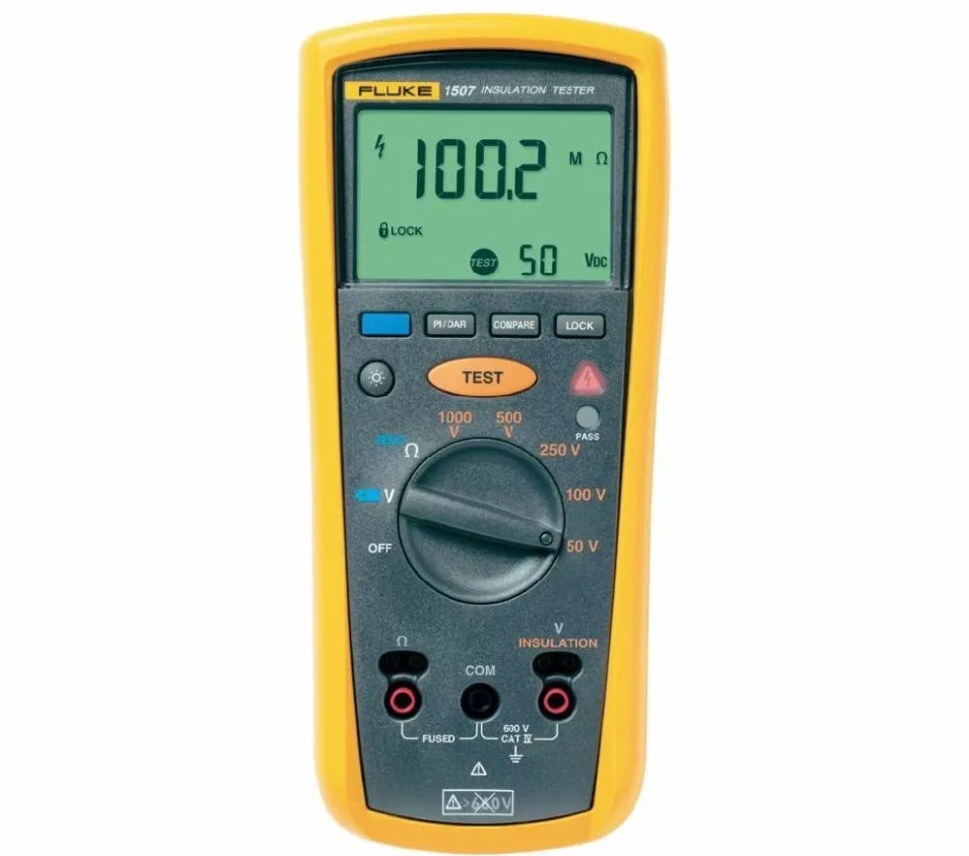
\includegraphics[width=0.3\textwidth]{img/Megahometro megger.png}%
            \label{fig:imagen2}
        }\hfill
        \subfloat[Amperimetro Analogico.]{%
            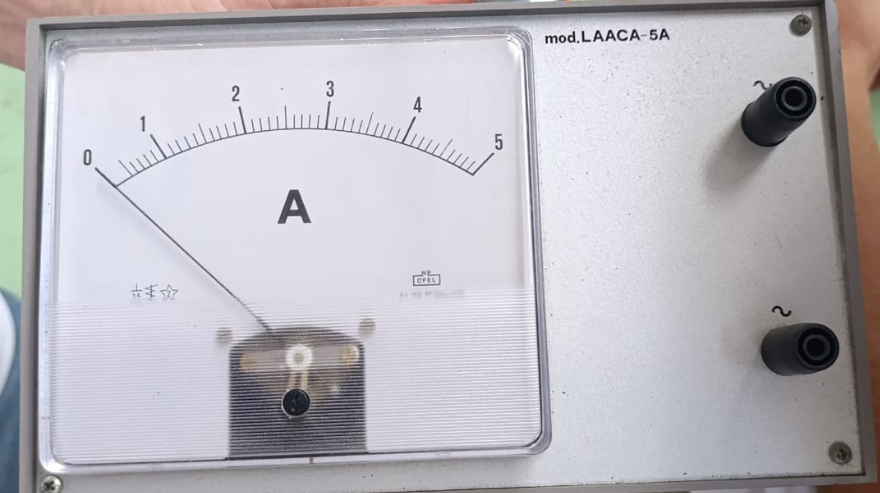
\includegraphics[width=0.3\textwidth]{img/Amperimetro Analogico.png}%
            \label{fig:imagen3}
        }
        \caption{Conjunto de imágenes}
        \label{fig:conjunto_imagenes}
    \end{figure}
    
\end{comment}

\newpage
\section{INTRODUCCIÓN }
Los transformadores electricos son instrumentos empleados para el transporte de energia a largas distancias y aprovechamiento de dicha energia para diversas tareas.En este informe se aborda una descripcion del proceso realizado durante la practica en el laboratorio donde se tomaron diferentes medidas para tener algunos parametros del transformador monofasico y se identificaron las borneras de dicho transformador, se analizan los valores obtenidos en la prueba de aislamiento, la relación de transformación y la polaridad del transformador. tambien se describen alternativas a los metodos empleados en la practica como es el caso de la polaridad del transformador y el metodo de la descarga iductiva o de C.C..\\ \newline Estas mediciones son esenciales para evaluar el estado operativo del transformador y detectar posibles fallas en el aislamiento que podrían comprometer su funcionamiento seguro y eficiente para el transporte a largas distancias o el uso residencial.

\section{CONCLUSIONES}
Se logro satisfactoriamente comoprender como se realiza las diferentes conexiones para medir parametros como son la relacion de transformacion, la polaridad y la resistencia de aislamiento de un transformador monofasico, ademas de eso se logro comprender la importancia de la correcta conexion de los instrumentos de medicion para obtener resultados confiables y precisos. 

\begin{thebibliography}{99}
% Aquí puedes incluir tus referencias
\bibitem{ref1} Autor. Título del libro. Editorial, Año.
\bibitem{ref2} Autor. Título del artículo. Revista, Año.
\end{thebibliography}


\end{document}
